\documentclass[11pt,a4paper]{article}
\usepackage[margin=2.3cm]{geometry}
\usepackage[T1]{fontenc}
\usepackage[utf8]{inputenc}
\usepackage{lmodern}
\usepackage{amsmath}
\usepackage{microtype}
\usepackage{parskip}
\usepackage{graphicx}
\usepackage{booktabs}
\usepackage{array}
\usepackage{longtable}
\usepackage{xcolor}
\usepackage{listings}
\usepackage{tikz}
\usetikzlibrary{arrows.meta,positioning,shapes.geometric,fit,backgrounds}
\usepackage{caption}
\usepackage{float}
\usepackage{enumitem}
\usepackage[hidelinks]{hyperref}

\lstset{basicstyle=\ttfamily\small,breaklines=true,columns=fullflexible,keepspaces=true,
        backgroundcolor=\color{gray!8},frame=single,framerule=0pt,xleftmargin=0.6em,xrightmargin=0.6em}
\newcommand{\file}[1]{\path{#1}}
\newcommand{\PSNR}{\mathrm{PSNR}}
\setlist{nosep}

\title{BitSemCom + GRAND: a guide to the repository}
\author{Safaa Salman}
\date{November 2026}

\begin{document}
\maketitle

\begin{abstract}
This document explains, in plain language, what is in the \texttt{BitSemCom} repository, how one image
travels through the system, what every folder and script does, where the results are, and which
conventions you must know before touching the code. It is written for students who join the project.
The step-by-step commands are in the \texttt{README.md} at the repository root; this guide explains
what those commands do. The numbers we measured are in the companion document
\emph{BitSemCom + GRAND: results so far}.
\end{abstract}

\tableofcontents

\section{What this repository is}

The repository has two layers.

\textbf{The original BitSemCom.} Bit-level semantic image communication from Shanghai Jiao Tong University
(arXiv 2510.26225). A Swin-transformer autoencoder (the ``WITT'' backbone) turns an image into a short
sequence of bits, the bits are sent over a noisy channel as QPSK symbols, and a second Swin network
rebuilds the image from what arrives. The authors call it \emph{semantic} because the network decides
what to put in the bits; nothing in the bitstream is a pixel value. This code is in \file{main.py},
\file{network/}, \file{data/}, \file{loss/} and \file{utils.py}, untouched.

\textbf{Our addition: a channel code decoded by GRAND.} The thesis question is whether an explicit
error-correcting code, decoded with GRAND (Guessing Random Additive Noise Decoding), improves the image
quality of such a system. We put a CRC code between the bit mapper and the semantic decoder, decode it
with ORBGRAND (the soft-input version of GRAND), and measure image quality with and without it, on
several channels, with several receivers, and also with GRAND inside the training loop. That code is in
\file{grand/}, \file{experiments/}, \file{train_bitsemcom.py} and \file{matlab/}.

Branch \texttt{main} holds the original code only; branch \texttt{grand-implementation} holds everything
described here.

\section{How one image travels through the system}

Figure~\ref{fig:pipeline} shows the path of one $256\times256$ image. The grey boxes are the original
BitSemCom, the orange boxes are what we added. Each box is explained below.

\begin{figure}[H]
\centering
\resizebox{\textwidth}{!}{%
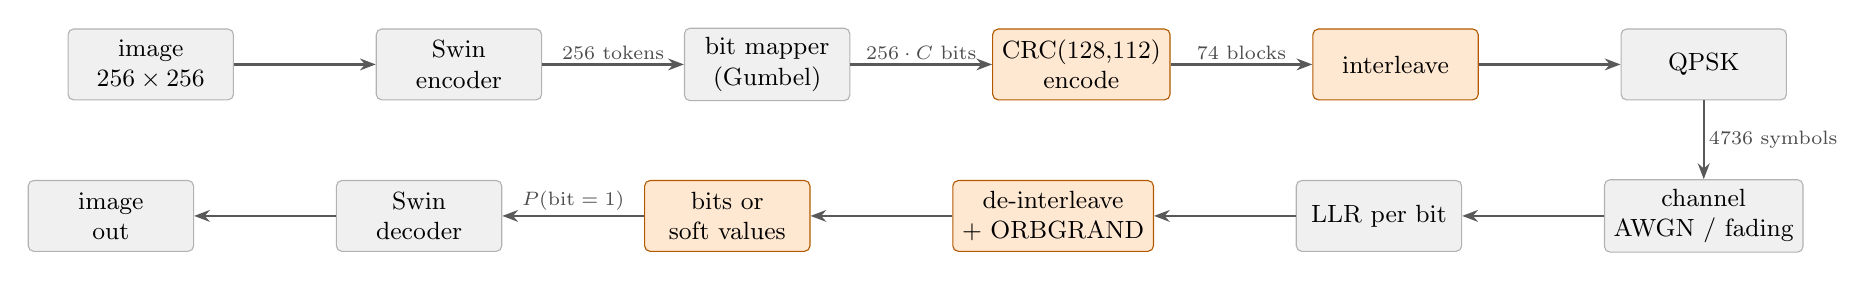
\begin{tikzpicture}[
  node distance=10mm and 18mm,
  box/.style={draw, rounded corners=2pt, minimum height=9mm, minimum width=21mm, align=center, font=\small, fill=gray!12, draw=gray!60},
  ours/.style={box, fill=orange!18, draw=orange!70!black},
  arr/.style={-{Stealth[length=2mm]}, thick, gray!70!black},
  lbl/.style={font=\scriptsize, text=gray!60!black, align=center, inner sep=1.5pt}
]
\node[box] (img) {image\\$256\times256$};
\node[box, right=of img] (enc) {Swin\\encoder};
\node[box, right=of enc] (bm) {bit mapper\\(Gumbel)};
\node[ours, right=of bm] (crc) {CRC(128,112)\\encode};
\node[ours, right=of crc] (il) {interleave};
\node[box, right=of il] (qpsk) {QPSK};
\node[box, below=of qpsk] (ch) {channel\\AWGN / fading};
\node[box, left=of ch] (llr) {LLR per bit};
\node[ours, left=of llr] (dil) {de-interleave\\+ ORBGRAND};
\node[ours, left=of dil] (p1) {bits or\\soft values};
\node[box, left=of p1] (dec) {Swin\\decoder};
\node[box, left=of dec] (out) {image\\out};
\draw[arr] (img) -- (enc);
\draw[arr] (enc) -- node[lbl, above] {256 tokens} (bm);
\draw[arr] (bm) -- node[lbl, above] {$256\cdot C$ bits} (crc);
\draw[arr] (crc) -- node[lbl, above] {74 blocks} (il);
\draw[arr] (il) -- (qpsk);
\draw[arr] (qpsk) -- node[lbl, right] {4736 symbols} (ch);
\draw[arr] (ch) -- (llr);
\draw[arr] (llr) -- (dil);
\draw[arr] (dil) -- (p1);
\draw[arr] (p1) -- node[lbl, above] {$P(\text{bit}=1)$} (dec);
\draw[arr] (dec) -- (out);
\end{tikzpicture}}
\caption{One image through the system for $C=32$. Grey: the original BitSemCom. Orange: the coded link we
added. Without the orange boxes the LLRs are turned into $P(\text{bit}=1)$ directly and handed to the
decoder; that is the original receiver.}
\label{fig:pipeline}
\end{figure}

\begin{description}[style=nextline]
\item[Encoder and tokens.] The Swin encoder downsamples the image by 16 in each direction, so a
$256\times256$ image becomes $16\times16=256$ \emph{tokens}, each a feature vector.
\item[Bit mapper and $C$.] For every token the bit mapper produces $C$ bits with a Gumbel-softmax
layer (\texttt{Resample\_Layer} in \file{network/network.py}). $C$ is the only size knob: $C=16$, 32, 64
give 4096, 8192, 16384 bits per image. The layer is stochastic: sampling it twice flips about 5\% of
the bits, and the decoder was trained to live with that.
\item[CRC code (ours).] The bits are cut into blocks of $k=112$ and each block gets 16 parity bits from
a CRC polynomial (Koopman notation \texttt{0x9eb2}), giving codewords of $n=128$ bits, rate 0.875. The
code is \emph{systematic}: the codeword is the 112 data bits followed by the 16 parity bits. For $C=32$
the 8192 bits are padded to 74 blocks (9472 coded bits), 16\% more than uncoded.
\item[Interleaver (ours).] A fixed pseudo-random permutation of all coded bits, known to both sides.
In fading, a deep fade wipes out a whole token; after interleaving its bits are spread over many
codewords and many tokens, which both the code and the semantic decoder handle far better.
\item[QPSK and channel.] Two bits per symbol, Gray mapping, exactly the mapping of the original
\texttt{QPSK\_soft}. Channels: AWGN, or block Rayleigh fading with one complex gain per block of
symbols (\texttt{fade8} = one gain per 8 symbols = one $C=16$ token). Optional channel-state errors:
the receiver may assume an SNR that is wrong by $\pm3$ dB, or use a noisy channel estimate.
\item[LLR.] For every bit the receiver computes a log-likelihood ratio. Convention everywhere in this
repository and in Duffy's code: \textbf{positive LLR means bit 0}. The original receiver converts it to
$P(\text{bit}=1)=\sigma(-\mathrm{LLR})$ and gives that number to the decoder.
\item[ORBGRAND (ours).] GRAND does not decode the code directly; it guesses the \emph{noise}. It sorts
the bits by reliability $|\mathrm{LLR}|$, flips the least reliable bits first in a fixed order of
patterns (the ``landslide'' pattern generator), and after each guess checks whether the result is a
valid codeword ($Hc=0$). The first valid codeword wins. If no codeword is found within the \emph{guess
budget} the block is \emph{abandoned}. If a wrong codeword passes the check the block is
\emph{miscorrected}: the decoder then receives confidently wrong bits, which is the one way GRAND can
hurt.
\item[What the decoder receives (ours).] Decoded blocks: exact 0/1 values of their 112 data bits.
Abandoned blocks: the plain soft values the uncoded receiver would have used (\emph{soft fallback};
\emph{hard fallback} gives 0/1 decisions instead). The padding is dropped and the $256\cdot C$ values
go to the Swin decoder, which cannot tell which receiver produced them.
\end{description}

\section{Repository map}

\begin{longtable}{p{0.34\textwidth} p{0.6\textwidth}}
\toprule
Path & What it is \\
\midrule
\endhead
\file{main.py} & the original training and test script (two stages: error-free channel, then noisy channel). Hard-coded dataset paths in its \texttt{config} class. Needs \texttt{lpips}, \texttt{thop}, \texttt{tensorboardX} and a CUDA GPU. \\
\file{network/network.py} & the \texttt{WITT} model: encoder, bit mapper (\texttt{Resample\_Layer}), \texttt{QPSK\_soft} (channel + LLR + $P(1)$), decoder. \\
\file{network/encoder.py}, \file{decoder.py}, \file{modules.py} & Swin blocks. \file{network/channel.py} is unused by the bit path. \\
\file{data/datasets.py}, \file{loss/distortion.py}, \file{utils.py} & loaders, MS-SSIM, logging helpers of the original code. \\
\file{train_bitsemcom.py} & our trainer: fixed step budget, warmup + cosine learning rate, random SNR per batch, validation every $N$ steps, best checkpoint, resume; \texttt{-{}-grand} puts the coded link + ORBGRAND into the loop. \\
\file{grand/codes.py} & builds CRC and random linear codes: generator matrix $G=[I\,|\,P]$, parity-check matrix $H=[P^T\,|\,I]$, \texttt{encode}, \texttt{is\_codeword}. \\
\file{grand/orbgrand.py} & ORBGRAND in pure numpy (basic and 1-line variants, landslide generator), port of Duffy's MATLAB. \texttt{ORBGRAND(H, max\_queries).decode(llr)} returns (word, guesses, abandoned). \\
\file{grand/selftest.py}, \file{grand/validate_duffy.py} & self-test; reproduction of the block error rate curves shipped with GRAND-MATLAB. \\
\file{experiments/bitsemcom_io.py} & builds the model without importing \file{main.py}; loads checkpoints with a strict key check; encodes images to bits and decodes probabilities to images. \\
\file{experiments/channel_coding.py} & the coded link (\texttt{CodedLink.transmit}): pad, encode, interleave, QPSK, channel with CSI errors, LLR, ORBGRAND, fallback, statistics. Also the uncoded QPSK channel in numpy. \\
\file{experiments/torch_channel.py} & the same uncoded QPSK channel in torch, differentiable, used in training. \\
\file{experiments/grand_layer.py} & \texttt{GrandChannel}: GRAND inside training. Forward value = the coded link's output; gradient = the uncoded soft channel's Jacobian (section~\ref{sec:training}). \\
\file{experiments/conditions.py} & the grammar of channel-condition names (section~\ref{sec:conditions}). \\
\file{experiments/metrics.py} & PSNR, MS-SSIM, LPIPS (AlexNet), CLIP ViT-B/32 cosine similarity. \\
\file{experiments/run_grand.py} & round-1 sweep runner: one model, several SNRs, all receivers; one JSONL row per (image, SNR, receiver). \\
\file{experiments/evaluate.py} & round-2 sweep runner: several models $\times$ conditions $\times$ SNRs $\times$ receivers, four metrics, optional MATLAB decoding, example images. \\
\file{experiments/plot_llr.py} & the LLR study: what the decoder and GRAND receive under each condition. \\
\file{experiments/plot_results.py}, \file{plot_training.py}, \file{plot_review_gains.py}, \file{plot_style.py} & all figures: quality curves, coding gains, GRAND block statistics, training curves, the paired-gain charts of the review, example strips; one shared style. \\
\file{experiments/summarize.py} & markdown tables from round-1 JSONLs. \\
\file{experiments/bit_importance.py}, \file{channel_importance.py} & round-1 diagnostics: flip a fraction of bits (random, most confident, least confident, whole tokens, per channel) and measure the PSNR drop. \\
\file{experiments/grand_verify.py}, \file{grand_backend.py}, \file{matlab/} & export of a test set of LLR blocks, bit-exact comparison with Duffy's MATLAB code, and a decoding backend that routes every ORBGRAND call through MATLAB or Octave. \\
\file{experiments/make_kodak_patches.py} & makes the 24 centre $256\times256$ crops of Kodak used everywhere. \\
\file{BitSemCom_Colab.ipynb} & the round-2 experiments as Colab cells (models, data and results on Google Drive). \\
\file{results/} & raw results, tables, figures, training logs (section~\ref{sec:results}). \\
\file{docs/} & the two markdown reports, their figures, and these LaTeX documents. \\
\file{Pretrain/}, \file{datasets/} & checkpoints and images; git-ignored, see the README for where to get them. \\
\bottomrule
\end{longtable}

\section{Training: without and with GRAND}
\label{sec:training}

\subsection{The original recipe (\texttt{main.py})}

The authors train in two stages. Stage 1 trains the autoencoder with an error-free channel (the
\texttt{WITT\_BitSC\_C*} checkpoints). Stage 2 starts from stage 1 and fine-tunes with
\texttt{-{}-pass\_channel}: each epoch draws one integer SNR between \texttt{-{}-snr\_min} and
\texttt{-{}-snr\_max}, sends the bits through \texttt{QPSK\_soft} and trains the whole network on the
reconstruction MSE. The learning rate is stepped down by \texttt{-{}-decay} every \texttt{-{}-step} epochs
to \texttt{-{}-min\_lr}. The loop never ends by itself (ten million epochs); a checkpoint is written every
20 epochs to \texttt{history/BitSC\_Prob/<timestamp>/models/}. Our starting checkpoints
\texttt{Pretrain/BitSemCom\_C\{16,32,64\}\_stage2\_ep*.model} are stage-2 models trained this way on Colab,
with SNR in $[-3, 6]$ dB.

\subsection{Our trainer (\texttt{train\_bitsemcom.py})}

The supervisor asked for a benchmark ``trained properly'': a fixed budget of 30{,}000 steps, AdamW,
500 warmup steps then cosine decay from $10^{-4}$ to $10^{-6}$, gradient clipping, SNR drawn per batch
from the continuous range $[0, 10]$ dB, bf16 autocast for the Swin blocks, validation every 1000 steps
on the 24 Kodak crops at 0, 3, 6 and 10 dB with fixed seeds, and the best checkpoint kept. One training
step is:

\begin{enumerate}
\item image $\to$ encoder $\to$ bit mapper $\to$ bits (the Gumbel layer passes a gradient through its own
straight-through trick);
\item channel: the uncoded torch QPSK (\texttt{channel\_uncoded}) or, with \texttt{-{}-grand}, the GRAND
channel (\texttt{GrandChannel.transmit});
\item $P(1)$ $\to$ decoder $\to$ MSE on the 0--255 scale $\to$ backward $\to$ AdamW step.
\end{enumerate}

\subsection{How GRAND is put inside the loop}

\texttt{GrandChannel.transmit} (\file{experiments/grand_layer.py}) moves the batch's bits to numpy,
sends each image to a worker process, and the worker runs the very same \texttt{CodedLink.transmit}
that evaluation uses (CRC encode, interleave, QPSK, channel, LLR, ORBGRAND with budget 2000, soft
fallback). The $P(1)$ values come back as a tensor of the same shape the uncoded channel would return,
so the decoder cannot tell which channel it is attached to.

Encoding, interleaving and ORBGRAND are not differentiable. The trainer therefore pushes the same bits
through the uncoded torch channel a second time (fresh noise, same settings) and combines the two:
\[
p_1 \;=\; \operatorname{stopgrad}(p_1^{\text{GRAND}}) \;+\; \bigl(p_1^{\text{soft}} - \operatorname{stopgrad}(p_1^{\text{soft}})\bigr).
\]
The value is exactly the GRAND output (the bracket is zero) while the gradient is the uncoded soft
channel's Jacobian, so the encoder is trained by the same gradient path as in the benchmark run; only
the forward signal the decoder sees differs (\texttt{-{}-grand\_grad soft}, the default;
\texttt{identity} is plain straight-through). The block statistics of every step (abandoned,
miscorrected, guesses, decode time) go to \file{log.csv}. In the run we made, about half of the blocks
were abandoned and 1.5\% miscorrected, flat for all 30k steps, because with fixed-power QPSK the encoder
has no handle on which blocks decode.

\section{Evaluation}

\subsection{Receivers}

Every receiver gets the same semantic bits and the same channel noise for a given (image, SNR, seed),
so all comparisons are paired: the difference between two receivers on one image is a difference
between two runs that share everything except the receiver.

\begin{tabular}{p{0.26\textwidth} p{0.68\textwidth}}
\toprule
Name & What the semantic decoder receives \\
\midrule
\texttt{noiseless} & the exact bits: the ceiling for any channel code \\
\texttt{uncoded\_soft} & $P(\text{bit}=1)$ from the QPSK soft demodulator: the original BitSemCom receiver \\
\texttt{uncoded\_soft\_il} & the same, with the coded link's interleaver but no code: isolates the interleaving gain \\
\texttt{uncoded\_hard} & hard 0/1 decisions \\
\texttt{coded\_soft} & interleaver + CRC(128,112) + ORBGRAND, abandoned blocks fall back to the soft values \\
\texttt{coded\_hard} & the same, abandoned blocks fall back to hard decisions \\
\texttt{*\_ebn0}, \texttt{*\_noil} & round 1 only: coded path at equal energy per semantic bit; coded path without interleaver \\
\bottomrule
\end{tabular}

\subsection{Channel conditions}
\label{sec:conditions}

Condition names (\file{experiments/conditions.py}) are tokens joined by underscores:
\texttt{awgn} or \texttt{fade<N>} ($N$ symbols per fading block; \texttt{fade1} is fast fading,
\texttt{fade8} one gain per 8 symbols); \texttt{over<X>} / \texttt{under<X>}: the receiver assumes an SNR
$X$ dB too high / too low; \texttt{h<Y>}: channel-estimate error of variance $Y$ (fading only);
\texttt{rnd<X>}: SNR error drawn uniformly in $[-X, X]$ per transmission. The round-2 sweep used
\texttt{awgn}, \texttt{awgn\_over3}, \texttt{awgn\_under3}, \texttt{fade8}, \texttt{fade8\_h0.1} at
$E_s/N_0$ from 0 to 12 dB in 2 dB steps.

\subsection{The two sweep runners}

\file{experiments/run_grand.py} (round 1) takes one model and one channel and writes one JSONL row per
(image, SNR, receiver) with PSNR, MS-SSIM and, for coded receivers, the block statistics.
\file{experiments/evaluate.py} (round 2) takes several models (\texttt{-{}-ckpt name=file}), a list of
condition names, SNRs and receivers, adds LPIPS and CLIP, can save example reconstructions
(\texttt{-{}-save\_images}), and can decode through MATLAB (\texttt{-{}-grand\_backend}). The guess budget
(\texttt{-{}-budget}) matters: the main sweep uses 2000, the budget the GRAND model was trained with; a
second sweep uses 100{,}000.

Each JSONL row has the keys \texttt{model}, \texttt{image}, \texttt{C}, \texttt{snr}, \texttt{condition},
\texttt{channel}, \texttt{fade\_block}, \texttt{snr\_err\_db}, \texttt{h\_err\_var}, \texttt{path},
\texttt{channel\_snr}, \texttt{payload\_bits}, \texttt{psnr}, \texttt{msssim}, \texttt{lpips},
\texttt{clip} and, for coded receivers, \texttt{n}, \texttt{k}, \texttt{blocks}, \texttt{coded\_bits},
\texttt{symbols}, \texttt{ber\_channel}, \texttt{ber\_after}, \texttt{bler\_channel},
\texttt{bler\_after}, \texttt{abandon\_rate}, \texttt{miscorrect\_rate}, \texttt{avg\_queries},
\texttt{max\_queries\_seen}, \texttt{decode\_time\_s}.

\subsection{Metrics}

PSNR is the headline number (mean over the 24 images; differences below about 0.03 dB are noise).
MS-SSIM and LPIPS (AlexNet; lower is better) are computed for every image. CLIP similarity (ViT-B/32
cosine similarity between the two images) was meant as a ``semantic'' metric but is too noisy on 24
images to separate receivers.

\subsection{Figures}

\file{plot_results.py} draws, per condition, the four metrics against SNR for every model and receiver
(\file{quality_*.png}), the coding gain against the plain receiver (\file{gain_*.png}) and against the
interleaver-only receiver (\file{gain_*_vs_il.png}), and the GRAND block statistics
(\file{grand_*.png}); it also writes \file{summary.md}. \file{plot_training.py} draws the training
curves from \file{log.csv}/\file{val.csv}. \file{plot_review_gains.py} draws the paired-gain bar charts
of the review (room up to perfect bits against the coded gain, GRAND-trained minus benchmark, cost of
imperfect CSI, budget 2000 against 100{,}000, example reconstruction strips).

\section{The GRAND package}

\file{grand/codes.py}: \texttt{make\_crc(k, poly)} builds the systematic generator matrix $G$ ($k\times
n$) and parity-check matrix $H$ ($(n-k)\times n$) from a CRC polynomial; \texttt{make\_rlc} builds a
random linear code; \texttt{encode(u, G)} is $uG \bmod 2$. \file{grand/orbgrand.py}:
\texttt{ORBGRAND(H, max\_queries, variant)} with \texttt{decode(llr)} and \texttt{decode\_many}. Syndromes
are packed into 64-bit integers and the noise patterns are cached, so the decoder runs at roughly two
million guesses per second in pure numpy. \texttt{budget\_mode='level'} reproduces the per-weight-level
budget check of Duffy's MATLAB code, so a block may use up to about 15\% more guesses than the nominal
budget; this mode is used everywhere numbers are compared with the reference.

The port was validated twice: \file{grand/validate_duffy.py} reproduces the block error rates and
average guess counts of the \texttt{RESULTS/*.mat} files shipped with GRAND-MATLAB within Monte Carlo
noise; and \file{experiments/grand_verify.py} exports 740 real LLR blocks for a bit-exact comparison
with the unmodified MATLAB functions (\file{matlab/verify_port.m}). The second check has not yet been
run with a real MATLAB installation; the Octave attempt stopped on \texttt{cumsum(d,'reverse')}, which
Octave lacks, and \file{matlab/octave_compat/cumsum.m} is an untested stand-in.

\section{Data, checkpoints and results}
\label{sec:results}

\textbf{Data.} Kodak (24 images) at \file{datasets/kodak_full}, and the centre $256\times256$ crops at
\file{datasets/kodak_patches256} made by \file{experiments/make_kodak_patches.py}; every reported
number is on those 24 crops. DIV2K train HR (800 images) is used for training only.

\textbf{Checkpoints} (\file{Pretrain/}, not in git): the authors' stage-1 models; the stage-2 models
that all experiments start from, named \texttt{BitSemCom\_C<C>\_stage2\_ep*.model} for $C=16$, 32, 64;
and the round-2 models \file{runs/C32_bench/best.model} and \file{runs/C32_grand/best.model}.

\textbf{Results} (\file{results/}): round-1 JSONLs \file{C16_*}, \file{C32_*}, \file{C64_*} with their
markdown tables \file{summary_*.md} and the diagnostics \file{bit_importance_*.md},
\file{channel_importance_*.md}; round-2 sweeps \file{eval_C32.jsonl} (12{,}600 rows, budget 2000) and
\file{eval_C32_b1e5.jsonl} (budget 100{,}000); training logs in \file{train_logs/} (\file{log.csv},
\file{val.csv} and the console output of the benchmark run, the GRAND run and the abandoned first GRAND
attempt); all figures in \file{figures/}; the MATLAB test-set description in \file{grand_verify/}.
Example reconstructions (\file{results/images_C32/}) and the test set itself (\file{testset.mat}) are
git-ignored and live on the project Drive.

\textbf{Reports} (\file{docs/}): \file{grand_results.md} (round 1) and \file{grand_review.md} (round 2,
with its figures in \file{docs/figures/grand_review/}), plus this guide and the results document in
\file{docs/latex/}.

\section{Conventions you must know}

\begin{itemize}
\item \textbf{LLR sign.} Positive LLR means bit 0, in BitSemCom, in Duffy's code and in ours. The
decoder consumes $P(\text{bit}=1)=\sigma(-\mathrm{LLR})$, never bits and never LLRs.
\item \textbf{SNR.} Always $E_s/N_0$ per QPSK symbol in dB. The raw bit error rate is
$Q(\sqrt{E_s/N_0})$: 16\% at 0 dB, 5.8\% at 4 dB, 2.3\% at 6 dB, 0.6\% at 8 dB. Duffy's BPSK curves at
$E_b/N_0 = x$ correspond to this code's QPSK at $E_s/N_0 = x + 3$ dB plus the rate term.
\item \textbf{Equal $E_b/N_0$} for a rate-$R$ code means running the coded path at
$E_s/N_0 + 10\log_{10} R$, i.e. $-0.58$ dB for 112/128.
\item \textbf{Pairing.} The same (image, SNR, seed) gives the same bits and the same noise for every
receiver; report paired differences with their standard error over the 24 images.
\item \textbf{Budgets.} Evaluate a GRAND-trained model at the budget it was trained with (2000); a
larger budget turns abandonments into miscorrections.
\item \textbf{Code specs} are strings: \texttt{crc:0x9eb2:128:112} (CRC polynomial, $n$, $k$),
\texttt{rlc:128:104:0} (random linear code, $n$, $k$, seed).
\end{itemize}

\section{The most useful commands}

All commands, with the data and checkpoint setup, are in the README. The ones used most often:

\begin{lstlisting}
python grand/selftest.py
python experiments/run_grand.py --C 16 --snrs 2,4,5,6,7,8,10 --code crc:0x9eb2:128:112
python experiments/plot_llr.py --C 32 --limit 8 --snrs 0,4,8,12 --conditions awgn,awgn_over3,awgn_under3,fade8,fade8_h0.1,fade1 --budget 100000 --out results/figures
python train_bitsemcom.py --C 32 --train_dir datasets/DIV2K_train_HR --val_dir datasets/kodak_patches256 --steps 30000 --out runs/C32_bench
python train_bitsemcom.py --C 32 --train_dir datasets/DIV2K_train_HR --val_dir datasets/kodak_patches256 --steps 30000 --grand crc:0x9eb2:128:112 --grand_budget 2000 --out runs/C32_grand
python experiments/evaluate.py --C 32 --ckpt bench=runs/C32_bench/best.model --ckpt grand=runs/C32_grand/best.model --snrs 0,2,4,6,8,10,12 --conditions awgn,fade8 --paths noiseless,uncoded_soft,uncoded_soft_il,uncoded_hard,coded_soft --budget 2000 --out results/eval_C32.jsonl
python experiments/plot_results.py results/eval_C32.jsonl --out results/figures
python experiments/plot_review_gains.py results/eval_C32.jsonl --b1e5 results/eval_C32_b1e5.jsonl --out docs/figures/grand_review
\end{lstlisting}

\section{Glossary}

\begin{description}[style=nextline]
\item[Semantic bits] The bits the bit mapper produces; the network decides what they mean.
\item[Token] One of the 256 feature vectors the encoder produces for a $256\times256$ image; each becomes $C$ bits.
\item[LLR] Log-likelihood ratio of one bit: how sure the receiver is, and in which direction (positive = bit 0).
\item[Soft value / $P(1)$] The probability that a bit is 1, computed from the LLR. ``Soft'' receivers keep it; ``hard'' receivers round it to 0 or 1.
\item[Systematic code] A code whose codeword contains the data bits unchanged, followed by parity bits.
\item[GRAND / ORBGRAND] Decoding by guessing the noise pattern, most likely first, and checking each guess against the code. ORBGRAND orders the guesses by the bit reliabilities.
\item[Guess budget] The maximum number of guesses per block before the decoder gives up.
\item[Abandoned block] A block where the budget ran out; passed on as soft values (harmless).
\item[Miscorrected block] A block where a wrong codeword passed the check; passed on as confidently wrong bits (harmful).
\item[Interleaver] A fixed shuffle of bit positions that spreads a burst of errors over many codewords and tokens.
\item[Block fading] A channel whose gain is constant over a block of symbols and changes between blocks.
\item[CSI] Channel state information: what the receiver believes about the SNR and the channel gain.
\item[Paired difference] The difference between two receivers on the same image with the same bits and noise, averaged over images.
\end{description}

\end{document}
